%%%%%%%%%%%%%%%%%%%%%%%%%%%%%%%%%%%%%%%%%%%%%%%%%%%%%%%
% A template for Wiley article submissions.
% Developed by Overleaf.
%
% Please note that whilst this template provides a
% preview of the typeset manuscript for submission, it
% will not necessarily be the final publication layout.
%
% Usage notes:
% The "blind" option will make anonymous all author, affiliation, correspondence and funding information.
% Use "num-refs" option for numerical citation and references style.
% Use "alpha-refs" option for author-year citation and references style.
\documentclass[alpha-refs]{wiley-article}
%\documentclass[blind,alpha-refs]{wiley-article}
\usepackage{xcolor}
\usepackage{siunitx}
\usepackage{apalike}
\usepackage{gensymb}
\usepackage{makecell}
\usepackage{csquotes}
\usepackage{graphicx}
\usepackage{listings}
\usepackage[T2A]{fontenc}
\usepackage[utf8]{inputenc}
\usepackage[english]{babel}
\usepackage[version=3]{mhchem}
%\usepackage{amsmath,amsfonts,amssymb,amsthm,mathtools} % AMS

\papertype{Original Paper}

\title{Cytoskeletal and motility changes in human umbilical cord MSCs associated with nuclear-cytoplasmic RhoА redistribution during replicative senescence}


% List abbreviations here, if any. Please note that it is preferred that abbreviations be defined at the first instance they appear in the text, rather than creating an abbreviations list.
\abbrevs{DMEM, Dulbecco's modified Eagle's medium; DOX, sodium deoxycholate; FBS, fetus bovine serum; FPLC, fast performance liquid chromatography; HRP, Horseradish Peroxidase; MSCs, mesenchymal stem cells; RCF, relative centrifugal force; PCA, principal component analisys; MSCWJ-1, human umbilical cord MSCs cell line; bTau, $\tau$-Kendall rank correlation coefficient; Rs, Spearman's R correlation coefficient; tM, Manders correlation coefficient; Rval, Pearson correlation coefficient; SD, standard deviation}

% Include full author names and degrees, when required by the journal.
% Use the \authfn to add symbols for additional footnotes and present addresses, if any. Usually start with 1 for notes about author contributions; then continuing with 2 etc if any author has a different present address.
\author[1\authfn{1}]{Danila Bobkov}
\author[2\authfn{2}]{Anastasia Polyanskaya}
\author[1\authfn{1}]{Anastasia Musorina}
\author[1\authfn{1}]{Ekaterina Lomert}
\author[1\authfn{1}]{Sergey Shabelnikov}
\author[1\authfn{1}]{Galina Poljanskaya}

% \contrib[\authfn{1}]{Equally contributing authors.}

% Include full affiliation details for all authors
\affil[1]{Institute of Cytology of the Russian Academy of Science, 194064 Tikhoretsky ave. 4, St-Petersburg, Russia }
\affil[2]{Peter the Great St. Petersburg Polytechnic University, Polytechnicheskaya, 29,  St.Petersburg, 195251, Russia}

\corraddress{Tikhoretsky ave. 4, St-Petersburg, 194064, Russia}
\corremail{bobkov@incras.ru}

\presentadd[\authfn{2}]{Peter the Great St. Petersburg Polytechnic University, Polytechnicheskaya, 29,  St.Petersburg, 195251, Russia}

\fundinginfo{This research received no external funding.}

% Include the name of the author that should appear in the running header
\runningauthor{Bobkov et al. Motility changes in aging MSCs}

\begin{document}

\maketitle

\begin{abstract}

  Here we provide evidence for changes in cell motility and organization of the contractile apparatus of human umbilical cord MSCs in the process of replicative senescence.
  The colocalization dynamics of myosin-9, alpha-actinin-4, and RhoA with F-actin and nuclei were examined in MSCWJ-1.
  Result shows that RhoA nuclear-cytoplasmic redistribution occurs during replicative senescence, with maximal RhoA nuclear localization at passage 15.
  At the same time point, a decrease in the colocalization of F-actin with myosin-9 and $\alpha$-actinin-4 was found, and myosin-9 was found in cytosolic extracts in the assembly-incompetent form.
  Using the automated system of intravital confocal cytometry we found that changes in cytoskeleton organization correlates with cell motility characteristics in MSCWJ-1.
  Quantitative analisys of MSCWJ-1 movements revealed decline in cell speed from 9 to 36 passage.
  Results of cytoskeloton structural analysis together with cell motility characteristics allows us to divide the process of replicative senescence into two stages.
  The first stage lasts from thawing to passage 15 and is characterized by the accumulation of actin-binding proteins in the assembly-incompetent forms, nuclear RhoA accumulation and increase in movement tortuosity.
  The second stage lasts from 15 passage to 36 passage is characterized by an increase in the structural integrity of the actin cytoskeleton, exit of RhoA and $\alpha$-Actinin-4 from nucleus and increase in movement straightness.

% Please include a maximum of seven keywords
\keywords{mesenchymal stem cells, \emph{cellular senescense}, actin cytoskeleton, myosin-9, $\alpha$-actinin-4, RhoA, cell motility}
\end{abstract}

\section{Introduction}

At present, the urgent task of cell biology is the isolation and comparative characterization of human MSCs isolated from various sources.
The importance of such studies stems from the features of the interaction of MSCs isolated from different tissues, with their characteristic microenvironment.
The origin or source of the MSC can determine their functional characteristics.
Analysis of the characteristics that are decisive in maintaining the status of MSCs, as well as a number of other characteristics responsible for the most important cellular processes, contributes to the deepening of basic knowledge of human MSCs, which is important both for understanding the mechanisms of biological processes in the cell and for expanding opportunities for using MSCs in regenerative medicine.
Due to the importance of MSCs for the functioning of the body, the mechanisms of MSC interaction with damaged tissues and organs are widely studied.
It has been shown that one of the most important mechanisms of action of various MSCs on damaged tissues is their ability to migrate to these sites and exert a trophic action due to the secretion of bioactive factors that alter the microenvironment of damaged cells and, thereby, improving tissue repair.
At present, the mechanisms of tissue repair using MSCs related to the production of cytokines and paracrine factors are widely discussed in the literature (\cite{phinney2007concise}; \cite{m2011mesenchymal}; \cite{guiducci2011bone}; \cite{gruenloh2011characterization}; \cite{huang2013effects}; \cite{luo2013mesenchymal}; \cite{ando2014stem}; \cite{hendijani2015human}; \cite{hendijani2015effect}; \cite{danieli2016testing}; \cite{julianto2016topical}; \cite{teixeira2017impact}; \cite{vulcano2016wharton}; \cite{zachar2016activation}).

Non-immortalized cell lines undergo a process of replicative senescence.
Replicative senescence is a complex process that can begin at the early passages and gradually increase in the process of long-term cultivation.
It is characterized by a significant decrease or cessation of proliferation, shortening of telomeres, morphological changes, increased $\beta$-galactosidase activity, increased expression of the tumor suppressor genes, decreased DNA repair and antioxidant activity of senescence cells, due to reduced expression of the corresponding genes, a number of epigenetic changes (\cite{wagner2008replicative}; \cite{kuilman2010essence}; \cite{redaelli2012cytogenomic}; \cite{estrada2013human}; \cite{savickiene2016senescence}; \cite{danisovic2017effect}; \cite{koltsova2018dynamics}; \cite{alessio2018mesenchymal}; \cite{krylova2018isolation}; \cite{niedernhofer2018nuclear}; \cite{truong2018characterization}; \cite{yu2018replicative}).
It is important to emphasize that senescence of MSCs may be associated not only with replicative senescence, which can be traced during long-term cultivation of MSCs in vitro, but also with factors external to MSCs.
Senescence mechanisms affect both MSCs and microenvironment.
In this regard, it is the interaction of MSCs and the microenvironment that ensures the age characteristics of MSCs.
One of the essential signs of replicative senescence is a decrease in cell motility or cell migration.
Violation of migration processes contributes to the deterioration of tissue repair (\cite{geissler2012functional}; \cite{bertolo2015vitro}; \cite{turinetto2016senescence}; \cite{zhang2018overexpression}).
Therefore, to use MSCs in regenerative medicine, it is necessary to know the nature of the process of replicative senescence in a particular line.

In order to find out how much cellular senescence can interfere with use of cells in biomedical work, it is important to  it is important to find out to what extent cell mobility is impaired during long-term cultivation.
Cell migration occurs through close contact with the extracellular matrix, on which cells are spread, and depends on the organization of the actin cytoskeleton.
In this regard, it is essential to study the role of senescence in the organization of the cytoskeleton.
Currently, studies on the effect of replicative senescence on cytoskeleton reorganization are at the stage of accumulation of experimental results.
There are a number of works describing molecular mechanisms and functional changes during the reorganization of the cytoskeleton during replicative senescence in different human and animal cell types (\cite{larsen2003phosphatases}; \cite{le2008regulation}; \cite{wang2009protein}; \cite{geissler2012functional}; \cite{ozcan2016unbiased}; \cite{turinetto2016senescence}; \cite{moujaber2019cellular}).
It is of considerable interest to analyze the effect of replicative senescence on cell motility and the reorganization of the actin cytoskeleton in the human MSC line, which has not been used in detail in such studies.
Actin cytoskeleton provide the driving forces for creating morphological diversity and the dynamics of mammalian cells (\cite{vasiliev1991polarization}).
Motor proteins, such as nonmuscle myosin isoforms, involved in maintaining cell shape, cell migration, interaction with the substrate and with other cells, processes of intracellular transport, as well as signalling and the regulation of gene expression (\cite{omelchenko2002mechanisms}).

In this work, we used MSCWJ-1 cells that were not previously investigated.
Little is known about how the structural aspects of these cells are modified as a result of replicative senescence.
Thus, the objective of this study is analysis of replicative senescence in the process of long-term cultivation of the MSCWJ-1 in connection whith the actin cytoskeleton state and the behavior of moving cells.
To analyze the state of the actin cytoskeleton, we selected two structural and one regulatory actin-binding proteins, myosin-9 and $\alpha$-actinin-4 as well as small GTPase RhoA.
Using immunofluorescence and confocal microscopy-based quantitative image cytometry techniques, we investigated changes in distribution of F-actin and actin-binding proteins  in conjunction with the registration of parameters characterizing cell motility.
In order to characterize the change in the composition of cytoplasmic protein complexes containing myosin-9 and beta-actin, we used liquid chromatography.

\section{RESULTS}

\subsection{$\beta$-Galactosidase activity}

During long-term cultivation (passages 7--36) within each passage, the culture was filled by homogeneous cell populations of fibroblast-like cells.
The results of $\beta$-galactosidase enzyme activity test shown in the table 1.
The proportion of stained cells naturally increases with passage number, which confirms the senescent status of MSCWJ-1.

\subsection{Colocalization analysis}

In order to follow the dynamics of the reorganization of the contractile apparatus during replicative senescence, we used the immunofluorescence method.
Using polyclonal antibodies against myosin-9, we performed initial passage screening.
Assuming that the cells in the neighboring passages are negligibly little different from each other, we fixed MSCWJ-1 and analyzed the myosin-9/F-actin colocalization at passages: 7, 9, 12, 15, 18, 21, 25, 27, 28, 35, 36.
The results shown in the figure 1.
In all spread cells, staining for myosin-9 reveals a characteristic striated pattern.
In addition to the striated pattern, myosin-9 was detected in lamellae as separate spots.
An increased number of cells with such spots was detected in preparations fixed at passages 15--20.
As can be seen in fig 3 (B) the colocalization of myosin-9 and F-actin decreases from high to moderate level during cultivation and reaches a minimum at passage 15.
Then, the colocolization rises to a very high level at passage 28, after which it again decreases during passage of cultivation to passage 36, which was our last time point.
The use of post hoc analysis revealed the most significant differences between groups associated with a decrease in colocalization at 15 and 18 passages (fig 3, C).
For further research, we decided that 9, 15, 28, and 36 passages would be key points.

The results of staining cells with $\alpha$-actinin-4 at passages 9, 15, 28, 36 shown in Fig. 2.
$\alpha$-Actinin-4 as well as myosin-9 was detected in cells at passages 9 and 36 in the form of striated patterns, less pronounced than in myosin-9, but nevertheless quite distinguishable.
At passage 15 $\alpha$-actinin-4 was detected as spotted pattern and in focal adhesions.
We studied the colocalization $\alpha$-actinin-4/F-actin and $\alpha$-actinin-4/nuclei.
The results are shown in Figure 2 (C), $\alpha$-actinin-4/nuclei colocalization decreases from moderate level to weak when moving from 28 to 36 passages.
The same decrease is observed in the transition from 9 to 15 passage in case of $\alpha$-actinin-4/F-actin colocalization.

RhoA was detected in the nucleus, along the stress in the perinuclear region, diffusely in the cytoplasm at passage 9, mainly in the nucleus at passage 15.
The colocalization of small GTPase RhoA with nuclei significantly increases from moderate to noticeable level while passage gone from 9 to 15, then decreases to the initial level at passage 28, and even more decreases to the weak level at passage 36 (Figure 3).
It should be noted that in almost half of the cells, the coefficient takes negative values, which indicates the complete absence of colocalization.

For a more detailed study of the detected phenomenon of nuclear-cytoplasmic shuttle, we used the analysis of 3D models performed in the nuclear region.
Figure 4 shows RhoA in the nucleus as 3D image slices based on Z-stacks.
In the XZ sections, it is noticeable that at the 9th passage, RhoA is distributed partly in the nucleus and partly in the cytolasm, at the 15th passage for the most part inside the nucleus and in the perinuclear region, and at the 36th passage only along stress fibrils and in the cytoplasm.

\subsection{Trajectory analysis}

The results of a quantitative analisys of 24-hour MSCWJ-1 movements show at figure 5.
Fig.5 (A) show characteristic frames from time laps of cell movement recording over 24 hours.
Сells are in sparse seeding, on each field of view several tracks are highlighted with colored lines.
Statistical analisys of the obtained trajectories are shown in Fig.5 (В).
Speed and path length significantly decreased with increase in passage number.
At the same time, the total distance traveled significantly decreases only when switching from 9 to 15 passages and 15 passage does not differ from 36.
The straightness of the trajectory increases significantly with the passage from passage 15 to 36.
The tortuosity of the trajectory increases with the transition from passage 9 to 15 and then decreases by passage 36 to a level significantly lower than it was at passage 9.
The numerical values obtained from the analysis are shown in the table 2.

\subsection{Gel chromatography}

Chromatographic analysis results shown at Fig 6.
Myosin-9 was detected at passage 9 mostly in high molecular weight fractions 3--4 (> 700 kDa), and to a lesser extent in fractions 7--9, approximately equal to the size of the monomeric protein (250 kDa).
At passage 15, the amount of myosin in fractions 3–--4 decreases, but the tail of the elution distribution is enriched: low molecular weight fractions are uniformly stained at a good signal level, starting from 10 to 14.
At passage 36, myosin-9 is detected mainly in 3---4 fractions.
$\beta$-Actin is detected mainly in the 10---11 fractions at passage 9.
But at 15 and 36 passages it also revealed in fractions 6---7.

\section{DISCUSSION}

Although a considerable amount of information is collected regarding replicative senescence since discovery that human cells cannot endlessly divide (\cite{hayflick1961serial}), little is known about the mechanisms of senescence in context of actin cytoskeleton structure and cell motility.
Although almost all MSCs in culture are in constant motion, one of the essential signs of replicative senescence is a decrease in cell motility.
Until now the cell motility characteristics has not been studied for senescent MSCs in details.
Both external and intrinsic factors control directionality of cell movement, therefore in is important to esitmate speed characteristics altogether with tortuosity (\cite{tiurin2013molecular}).

Previous studies on MSCWJ-1 showed that already at passage 13, in addition to increasing $\beta$-galactosidase activity, the average doubling time in cell population also increases.
Аt passage 28, in addition to above mentioned, other senescence signs also appear, such as changes in cell morphology, and a proliferation index decreases (\cite{koltsova2018dynamics}). Thus we selected MSCWJ-1  long cultivation as model for replicative senescence and examined two structural proteins (myosin-9 and $\alpha$-actinin-4) and one regulator responsible for actin cytoskeleton organization and cell motility --- small GTPase RhoA (\cite{wang2003regulation}, \cite{elliott2015myosin}).

Since mammalian nonmuscle myosin II is a kew protein in regulation cell motility (\cite{shutova2018mammalian}), we investigated its distribution at various passages.
We can interpret the spotted pattern observed at passages 15--20 in the case of myosin-9 and $\alpha$-actinin-4, as a partial disassembly of the cytoskeletal structures where we see the accumulation of actin-binding proteins in the form of individual particles, or multimolecular protein complexes.
Such multimolecular protein complexes, containind actin-binding proteins, for example tropomyosin and myosin-9, was described early (\cite{grenklo2008tropomyosin} ,\cite{bobkov2017effect}).
Apparently, the accumulation of myosin-9 in light molecular weight fractions after gel filtration, which we observe at passage 15, is due to the fact that the protein is in the assembly-incompetent form (\cite{vicente2009non}), which is also consistent with immunofluorescence data shown in this work.

$\alpha$-actinin-4 is interesting in that, in addition to well-characterized structural functions, it plays a role in cellular signaling.
It was shown that $\alpha$-actinins act as negative regulators of myosin stack formation \cite{hu2019reciprocal}.
On the other hand, $\alpha$-Actinin-4 was found in nuclei in association with NF-$\kappa$B transcription factor (\cite{bolshakova2007extra}, \cite{babakov2008rela}, \cite{lomert2018co}).
In addition to regulating cell motility, this protein plays a role in carcinogenesis of different localization (\cite{barbolina2008motility}, \cite{hsu2013alpha}).
$\alpha$-Actinin-4 was shown by \cite{an2016alpha} to induce the epithelial-to-mesenchymal transition and tumorigenesis.
Our results prove a decrease in the content of $\alpha$-actinin-4 in the nucleus at passage 36, which may indicate a decrease in the signaling function of this protein as a result of cellular senescence.
We assume that the detected changes in the myosin-9/F-actin and $\alpha$-actinin-4/F-actin colocalization reflect the phenomenon of partial disassembly of the cytoskeleton at passage 15, and assebly back at passage 28, which is may be characteristic for switching types of cell movement.

The small GTP-binding protein RhoA was initially shown to regulate the
assembly of focal adhesions and actin stress fibers in response to growth
factors (\cite{ridley1992small}).
It soon became clear that RhoA is one of the central regulators in the organization of the actin cytoskeleton (\cite{burridge2004rho}).
The Rho/ROCK signaling pathway regulates cell motility through the regulation of myosin-9 phosphorylation (\cite{elliott2015myosin}).
It is now clear that RhoA regulates the activity of several transcription regulators and also itself is localized to the nucleus by an as-yet-undiscovered mechanism, therefore the role that RhoA plays in the nucleus is currently being intensively studied (\cite{guilluy2011analysis}, \cite{kim2018regulation}).
Our results demonstrate that the nuclear cytoplasmic RhoA redistribution is involved in the process of cellular aging.

Since the actin cytoskeleton of non-muscle cells is a highly dynamic system and is constantly in the state of assembly / disassembly, it is very important to pay attention not only to the assembled structures reshown by various forms of F-actin stabilized by actin-binding proteins, but also to study the set of proteins corresponding to the disassembled cytoskeleton.
The distribution of proteins in fractions after gel filtration allows us to evaluate the structural features of the organization of a set of proteins that are not included in the cytoskeleton structures.
We investigated the distribution of $\beta$-actin in the fractions obtained by gel filtration of MSCWJ-1 cytosole extracts, because this isoactin is the main one in non-muscle cells (\cite{khaitlina2001functional}).
In "young" cells at passage 9, $\beta$-actin is detected as a single peak in fraction 11, which corresponds to the size of the monomeric protein.
As a result of cellular senescence, beta-actin forms additional peaks in fractions of 6-7 (approximately 500 kDa) at passages 15 and 36, which suggests that beta-actin forms complexes with other proteins.
It can be assumed that beta-actin forms stable cytoplasmic complexes with cofilin or other sequestering monomeric actin proteins.
Additional research including immunoprecipitation and mass-spectrometry are needed to clarify this assumption.

Thus, the totality of our results allows us to divide the process of replicative aging into two stages, which are followed on the background of a steady decrease in the speed of movement of cells.
The first stage lasts from thawing to passage 15 and is characterized by the accumulation of actin-binding proteins in the assembly-incompetent forms, nuclear RhoA accumulation and increase in movement tortuosity.
The second stage lasts from 15 passage to the end is characterized by an increase in the structural integrity of the actin cytoskeleton, exit of RhoA and $\alpha$-Actinin-4 from nucleus and increase in movement straightness.

\section{Experimental Procedures}

Trade names should be capitalized. The manufacturer's name should be followed by an address including town, (state, if USA) and country.

\subsection{Cell cultures: MSCWJ-1}

A line of human mesenchymal stem cells obtained from Varton's jelly of the human umbilical cord (MSCWJ-1) were obtained from "Collection of vertebrate cell cultures" of the Institute of Cytology of the Russian Academy of Sciences (St. Petersburg, Russia).
Main characteristics confirming the status of MSCs for MSCWJ-1, according to the requirements of the International Society for Cellular Therapy, were published previously (\cite{krylova2017derivation}, \cite{koltsova2018dynamics}, \cite{dominici2006minimal}; \cite{sensebe2010mesenchymal}).
MSCWJ-1 cells were cultured in growth medium containing 90\% DMEM/F12 medium (Biolot, Russia) and 10\% fetal bovine serum (FBS) (Hyclone, United States).
Cells were cultured in 5\% $CO_2$, $37^{\circ}  C$ and 90\% humidity conditions.
Microbiological analysis confirmed the absence of bacterial, fungal and mycoplasmal contamination in the resulting line.

\subsection{Replicative cell senescence}

The efficacy of the $\beta$-galactosidase enzyme was evaluated by the $\beta$-galactosidase enzyme activity.
MSCWJ-1 cells were grown in 3.5 cm Petri dishes until subconfluent formation.
Then the medium was removed and the cells were stained using a reagent kit (Senescence $\beta$-galactosidase staining kit; Cell Signaling, USA), according to the instructions.
In cells entering the phase of replicative senescence, the cytoplasm has a bright blue color.
The analysis was performed using an inverted microscope equipped with 60x objective (Nicon, Japan) on the 6th, 15th, 20th and 28th passages.
The percentage of stained cells in percent was determined by counting at least 1000 cells in different fields of view at one time point.
The results were processed statistically as described further.

\subsection{Immunofluorescence}

Coverslips with adherent cells were fixed in a 3\% solution of paraformaldehyde for 10 min at room temperature and permeabilized in a solution of 0.1\% TritonX-100 for 10 min at room temperature, then the coverslips with cells was poured with 1\% BSA solution for 20 min.
Rabbit polyclonal antibodies produced against the N-terminal peptide of the heavy chain of nonmuscle myosin IIA, rabbit polyclonal antibodies produced against the $\alpha$-actinin-4 and mouse monoclonal antibodies produced against the RhoA were used as the first antibodies.
Goat antibodies to the Alexa fluor 488 rabbit antigens (Invitrogen, USA) were used as second antibodies.
To visualize the actin cytoskeleton, cells were stained with rhodamine phalloidin for 20 min at room temperature and stained with DAPI with final concentration 1.5 $\mu$g/mL.
Preparations were made on ProLong Gold antifade reagent containing.
Cells were analyzed on a confocal microscope Leica SP8 (Germany).

\subsection{Colocalization analysis}

Colocalization coefficients were calculated using ImageJ version 1.52i using the Coloc 2 plugin (\cite{rueden2017imagej2}).
Raw 1024 x 1024 px images was in 72 dpi resolution.
For colocalization analysis images were opened in ImageJ, RGB channels were converted to 32 bit grayscale.
Data collected in two channels from manually adjusted ROIs in confocal images with MSCWJ-1 cells stained with polyclonal anti-myosin-9 antibodies and rhodamine phalloidin. Cells were fixed at passages: 7, 9, 12, 15, 18, 21, 25, 27, 28, 35, 36.
Cells were selected manually on merged image and ROI passed to Coloc2 plugin.
The bTau, Rval, Rs, tM1, tM2 colocalization coefficients were calculated and passed as CSV files to R environment (\cite{adler2008replicate}; \cite{bergholm2010analysis}).

We conducted PCA in order to identify the colocalization coefficient most suitable for our purposes.
The results shown in Supplementary.
Shortly, bTau and Rs coefficients shows very high correlation, tM1 and Rval coefficient shows moderate correlation.
Kruskal-Wallis rank sum test results suggest that bTau reflects changes in colocalization so well.
The PCA and factor analysis allowed us to conclude that bTau is the most suitable coefficient and in the future we use it for the analysis of cytoskeletal rearrangements.
In further analysis, the values of the bTau shown were interpreted in accordance with the Cheddock scale (see table 1 in Supplementary).

\subsection{Quantitative image cytometry and cell movement analysis}

Comparative analysis of cell movement characteristics relative to replicative senescence was performed using time-lapse movies.
For recording the movement of individual cells we used high-content Quantitative Image Cytometer CQ1 (Yokogawa, Japan) with spinning disk confocal technology (\cite{sakashita2015cq1}).
Cells were plated on 6-well dishes and stained with Hoechst 33342 (Invitrogen, USA).
Images were acquired during 24 h session with 405-nm laser and bright field illumination using 40x 0.95-NA dry objective lens.
All images had a 2560 x 2160 pixel resolution, with a pixel size equivalent to 1.3158 $\mu$m in x and y.
A set of x-y coordinates were obtained from images in ImageJ software with Manual tracking plugin.
Each cell was manually marked in the middle of the nucleus in each time point.
Only cells satisfying the following conditions were noted: the cell must be in the field of view in all frames, the cell does not divide.
Dividing cells were not counted.
Trajectories were obtained from from a set of x-y coordinates.
The resulting tracks were combined into a data frame and analyzed in the R environment using trajr package (\cite{mclean2018trajr}), which is a sutable toolkit for the numerical characterisation and analysis of the trajectories of moving cells.
Trajectory coordinates were read from a CSV data file, and then passed in to the trajectory analysis functions.
Trajectorys was resampled to 15 min fixed step lenght by rediscretization function using the algorithm described by Bovet \& Benhamou (\cite{bovet1988spatial}).
As a result of the analysis of the trajectories, we obtained the following parameters: total length of the trajectory, straight-line distance from the start to the end of the trajectory, mean and maximum speeds, straightness and sinuosity indexes.
To measure the straightness, or conversely, tortuosity, of trajectories, we used two indexes.
The simplest is straightness index and computed as D/L, where D is the distance from the start to the end of the trajectory, and L is the length of the trajectory.
This straightness index is a number ranging from 0 to 1, where 1 indicates a straight line.
The straightness index is considered to be a reliable measure of the efficiency of a directed walk, but inapplicable to random trajectories.
The sinuosity index defined by Benhamou (\cite{benhamou2004reliably}) may be an appropriate measure of the tortuosity of a random search path.
Sinuosity is a function of the mean cosine of turning angles, and is a corrected form of the original sinuosity index defined by Bovet and Benhamou (\cite{bovet1988spatial}).

\subsection{FPLC gel filtration}

Cytosolic cell extracts were prepared as described in our previos work, in short, formaldehyde cross-links were preliminarily created in the cells to protect the protein complexes from degradation, then the cells were lysed with a buffer preserving the F/G actin ratio (\cite{bobkov2017effect}).
For gel-chromatographic separation of cell extracts, an FPLC system (Pharmacia, Sweden) was used.
Signal detection was performed using Millichrome A-02 detection unit.
Elution was performed with elution buffer (150 mM NaCl, 50 mM Tris, pH 7.5, 0.02\% $NaN_3$).
The column was calibrated with the set of proteins shown in Supplementary.
We obtained cell extracts by lysis from a monolayer cell culture grown on 14 Petri dishes 9 cm in diameter.
In order to prevent the destruction of multimolecular protein complexes, in the first stage the medium in the plates was replaced with medium containing 10 $\mu$M formaldehyde, incubated for 10 minutes at $37^{\circ}$ C, then a solution of glycine at a concentration of 1.875 g per 200 ml was added to each cup PBS, incubated for 5-7 min at  $37^{\circ}$  C.
Subsequently, we washed the cups after glycine with a solution of PBS and poured 20 $\mu$l of protease inhibitor and 1 ml of lysis buffer was left for 1 min on ice.
Next, the method of sequential selection of cell extract was collected in the ependorf 1 ml of the sample.
The final stage of lizing was centrifugation for 10 min at 24000 RCF and freezing of the samples at -80 $\degree$ C.
The protein extract was filtered and applied to the column in a volume of 500 $\mu$l.
Fractions were collected on ice 1 ml each 2 min starting from time point determined by calibration set separation.
For protein sedimentation, 100 $\mu$l of 0.15\% DOX was added to the collected fractions and mixed vigorously, incubated for 10 minutes in a refrigerator, then 100 $\mu$l of 50\% TCA was added, mixed, incubated for 15 minutes in a freezer, and precipitated by centrifuging the protein for 30 minutes at 24000 RCF at $+4^{\circ}$ C.
The supernatant was removed, and cold 100\% acetone was added to the precipitate, mixed vigorously and incubated for 12 hours at $-20^{\circ}$ C.
A repeated washing with acetone was done, and then the protein was precipitated by centrifugation for 15 min at 24000 RCF at $+4^{\circ}$ C, the supernatant was collected, the precipitate was dried, and 2-fold sample buffer was added to the precipitate (125 mM Tris-HCl, pH 6.8, 4\% SDS, 10\% glycerol, 0.006\% bromo-phenol blue, 1.8\% $\beta$-mercaptoethanol).
Samples were heated for 10 minutes at $98^{\circ}$ C, probes were stored at -$20^{\circ}$ C before electrophoretic separation.

\subsection{Electrophoresis and western blot}

Proteins were separated by electrophoresis in a 12.5\%  polyacrylamide gel under denaturing conditions in the presence of SDS (\cite{laemmli1970cleavage}).
After electrophoresis, the gel was stained with Coomassie brilliant blue or carried out by Western blotting (\cite{towbin1979electrophoretic}).
Protein transfer from the gel to the Immobilon-P membrane (Millipore, United States) was carried out in Tris-glycine buffer pH 8.3, containing 10\% ethanol and 0.1\% SDS.
Western blotting was performed according to the ECL protocol (Amersham, USA).
After transferring, the membrane was washed for 20 minutes with PBS containing 0.1\% tween-20 and blocked non-specific binding sites with 5\% non-fat dry milk diluted in PBS for 1 hour.
The membrane was incubated with the first antibodies for 1 hour at room temperature three times. washed in PBS, stained with second antibodies for 1 h at room temperature.
Rabbit polyclonal antibodies produced against the N-terminal peptide of myosin-9, mouse monoclonal Anti-$\beta$-actin antibodies produced in mouse (clone AC-15) (Sigma, USA, city) were used as the first antibodies.
Rabbit antibodies to mouse antigens and goat antibodies to rabbit antigens conjugated with horseradish peroxidase (Sigma, USA) were used as second antibodies.
To enhance the signal in western blotting, SuperSignal substrate (Thermo Scientific, USA) was used.
Chemiluminescent radiation was recorded using a ChemiDoc system (Bio-Rad, USA).

\subsection{Description of statistical analysis methods}

The study materials were subjected to statistical processing using the methods of parametric and non-parametric analysis.
The accumulation, correction, systematization of the initial information were carried out in Microsoft Office Excel 2016 spreadsheets.
Statistical analysis was done using the free software computing environment R v. 3.5.3 (\cite{team2014r}).

The data obtained from $\beta$-Galactosidase activity assay were computed following the Wilson method to obtain 95 \% confidence intervals for binomial proportions (\cite{wilson1927probable}).

The data obtained from measurements of the colocalization coefficient were combined into variational series, in which the arithmetic mean values and SDs were calculated.
PCA, generalized linear model and maximum-likelihood factor analysis were performed if R environment (\cite{husson2010exploratory}, \cite{dobson2008introduction}, \cite{lawley1971factor}).
In the course of all-pairs comparisons of colocalization data post hoc multiple testing corrections were used to adjust the P-values: Mann-Whitney rank test, Bonferroni method, Scheffe’s, and Dunn’s tests).
The results were visualized using the free Python computing software environment and the scikit-posthocs package (\cite{Terpilowski2019}).

The data obtained from trajectory analysis were cleaned frome outliers: those observations that deviate from the 1st or 3rd quartile by more than one and a half interquartile range were deleted.
Quantitative indicators were evaluated for compliance with the normal distribution, for this purpose, the Shapiro – Wilk criterion  was used with $n > 170$ (\cite{shapiro1965analysis}; \cite{shapiro1972approximate}) as well as indicators of asymmetry and kurtosis (see Supplementary for details).
When comparing several samples of quantitative data with a distribution other than normal, Kruskal-Wallis criterion was used, which is a non-parametric alternative to single-factor analysis of variance (\cite{kruskal1952use}).
In the event that the calculated value of the Kruskal-Wallis criterion exceeded the critical one, the differences in the indicators were considered statistically significant (\cite{wilcoxon1992individual}).

Data and scrips used to generate the analyses are available via data repository on Github : \url{https://github.com/Dan609/myo}.


\section*{Author contributions}

Author1 and Author6 designed the research, analyzed the data, wrote the article.
Author2 carried out immunofluorescence and western blotting.
Author3 maintained cell line and made the $\beta$-galactosidase test.
Author4 carried out introvital confocal cytometry.
Author5 made the chromatographic separation.

\section*{Acknowledgements}

We are thankful to Dr. G. Stein and M. Vorobyov for their expert assistance in confocal microscopy.
We are thankful to S. Boykov for assistance in computational trajectory analysis.
We acknowledge I. Kropacheva and Dr. A. Koltsova for for technical help and general support.
We are thankful to Dr. XY for providing financial funding.
We appreciate Dr. Edvard's help in manuscript language proof reading.

\section*{Conflict of interest}
The authors declare no conflict of interest.


\bibliographystyle{apalike}
\bibliography{mybib}

\section*{Supporting Information}

Supplementary with statistical tests results.
Video files with cell tracking.

\section*{Tables}

\begin{table}[hbt!]
  \caption{$\beta$-galactosidase enzyme activity in MSCWJ-1 cells with limits of the 95\% confidence intervals for binomial proportions. Cells were fixed at different passages, then, using light microscopy, the number of cells stained for $\beta$-galactosidase was counted.}
  \label{tab}
\centering
\begin{tabular}{c|c|c}
 Passage Number & Cells stained,\% & Cell count  \\
 \hline
9 & 6.02 $\pm$ 0.72 & 3724 \\
15 & 20.55 $\pm$ 1.57 & 2404 \\
28 & 25.56 $\pm$ 2.72 & 1260 \\
36 & 37.62 $\pm$ 2.91 & 1026  \\
\end{tabular}
\end{table}

\begin{table}[hbt!]
  \caption{Cell movement trajectory analysis. MSCWJ-1 cells were stained with Hoechst33342 and seeded in 6-well plate at passages 9, 15, 36. From each well 40 fields of view were recorded within 24 hours on CQ1 automated cytometer, then tracks were manually collected from recorded images in ImageJ and passed to R for for further analysis. Mean $\pm$ SD shown for calculated movement parameters.
}
\centering
\begin{tabular}{|c|c|c|c|c|c|}
 \hline
 \thead{Passage} &\thead{Track count} & \thead{Mean Speed, $\mu$m/h} & \thead{Max Speed, $\mu$m/h} & \thead{Length, $\mu$m} & \thead{Distance, $\mu$m} \\
 \hline
 9 & 171 & 38.3 $\pm$ 15.2 & 164.9 $\pm$ 56.4 & 911.3 $\pm$ 362.4 &  278.2 $\pm$ 169.8 \\
 15 & 172 & 25.0 $\pm$ 11.1 & 127.9 $\pm$ 59.3& 595.1 $\pm$ 263.4 & 211.7 $\pm$ 162.8  \\
 36 & 178 & 18.3 $\pm$ 7.7 & 57.1 $\pm$ 27.8 & 431.6 $\pm$ 174.5 & 215.1 $\pm$ 156.4 \\
 \hline
\end{tabular}
\end{table}

\section*{Figure legends}

% bunch of good old long figure legends
\subsection*{Figure 1}
(A) Staining of F-actin (red) and myosin-9 (green) and nuclei (blue on merged images) in MSCWJ-1.
Cells were grown on glasses, fixed and permeabilised at passages 9, 15, 36.
Polyclonal antibodies against synthetic peptide corresponding to amino acids 1949-1960 of human nonmuscle myosin IIA and Alexa 488 secondary anti-rabbit antibodies were used for myosin-9 staining.
Hoechst33342 was used for nuclei staining.
Rhodamine phalloidin was used to stain actin cytoskeleton.
(B) Myosin-9/F-actin colocalization in MSCWJ-1.
Cells were grown on glasses, fixed and permeabilised at passages 7, 9, 12, 15, 18, 21, 25, 27, 28, 35, 36.
F-actin and myosin-9 were stained as previously indicated.
Ten fields of view were recorded using confocal microscopy, cells were manually selected on merged images and Kendall's colocalization coefficient (bTau) was measured in ImageJ, then data passed to R environment for statistical analysis.
Calculated means indicated by horizontal lines shown over jitter plots, each point indicate one observation.
The most interesting significant differences identified by the Wilcoxon test are indicated by p-values shown on square brackets.
(C) In the course of all-pairs comparisons of colocalization data post hoc multiple Mann-Whitney rank test was used to adjust the P-values.
The results were visualized using the free Python computing software environment and the scikit-posthocs package (\cite{Terpilowski2019})
For visualization of all significant differences in this dataset multiple pairwise comparison test was performed in Python environment.

\subsection*{Figure 2}
(A) Staining of F-actin (red) and $\alpha$-actintin-4 (green) and nuclei (blue on merged images) in MSCWJ-1.
Cells were grown on glasses, fixed and permeabilised at passages 9, 15, 36.
Polyclonal antibodies against human $\alpha$-actintin-4 and Alexa 488 secondary antibodies were used for $\alpha$-actintin-4 staining.
Hoechst33342 was used for nuclei staining.
Rhodamine phalloidin was used to stain actin cytoskeleton.
$\alpha$-actintin-4/F-actin (B) and $\alpha$-actintin-4/nucleus (C) colocolization in MSCWJ-1.
Cells were grown on glasses, fixed and permeabilised at passages 9, 15, 28, 36.
F-actin and $\alpha$-actintin-4 were stained as previously indicated.
Ten fields of view were recorded using confocal microscopy, cells were manually selected on merged images and Kendall's colocalization coefficient (bTau) was measured in ImageJ, then data passed to R environment for statistical analysis.
Calculated means indicated by horizontal lines shown over jitter plots, each point indicate one observation.
Significant differences identified by the Wilcoxon test are shown as asterisks on square brackets (* p < 0.05, *** p < 0.001, **** p < 0.0001, ns --- not significant).
Boxplots with means indicated by horizontal lines shown over jitter plots, each point indicate one observation.
Kruskal-Wallis test p-values are indicated under each plot.

\subsection*{Figure 3}
(A) Cell stained with polyclonal antibodies against RhoA (green), rhodamine-phalloidin (red), and Hoechst33342 (blue).
Cells were grown on glasses, fixed and permeabilised at passages 9, 15, 36.
Polyclonal antibodies against synthetic peptide corresponding to amino acids 177-189 located near the C-terminus of human RhoA and Alexa 488 secondary antibodies were used for RhoA staining.
Hoechst33342 was used for nuclei staining.
Rhodamine phalloidin was used to stain actin cytoskeleton.
RhoA/nucleus (B) and RhoA/F-actin  (C) colocalization.
MSCWJ-1 fixed at passages 9, 15, 28 and 36.
RhoA/nucleus colocolization in MSCWJ-1.
Cells were grown on glasses, fixed and permeabilised at passages 9, 15, 28, 36.
RhoA and nuclei were stained as previously indicated.
Ten fields of view were recorded using confocal microscopy, cells were manually selected on merged images and Kendall's colocalization coefficient (bTau) was measured in ImageJ, then data passed to R environment for statistical analysis.
Calculated means indicated in boxplots by horizontal lines shown over jitter plots, each point indicate one observation.
Significant differences identified by the Wilcoxon test are shown as asterisks on square brackets (* p < 0.05, *** p < 0.001, **** p < 0.0001, ns --- not significant).
Kruskal-Wallis test p-values are indicated under each plot.

\subsection*{Figure 4}
Confocal view of RhoA in the nucleus.
Cells were grown on glasses, fixed and permeabilised at passages 9, 15, 36.
Polyclonal antibodies against synthetic peptide corresponding to amino acids 177-189 located near the C-terminus of human RhoA and Alexa 488 secondary antibodies were used for RhoA staining.
Hoechst33342 was used for nuclei staining.
Rhodamine phalloidin was used to stain actin cytoskeleton.
One characteristic cell were selected and Z-scanning was performed to obtain 70 confocal sections, images were used to generate 3D models in LeicaX software, slices show sections passing through the nucleus.
White scalebars equals to 10 $\mu$m on each image section.


\subsection*{Figure 5}
Cell movement trajectory analysis.
MSCWJ-1 cells were stained with Hoechst33342 and seeded in 6-well plate at passages 9, 15, 36.
Then cells were incubated for 4 h for adhesion and and the plate was transferred to CQ1 automated cytometer, where 40 fields of view were recorded within 24 hours from each well.
Tracks were manually collected from recorded images in ImageJ and passed to R for for further analysis.
(A) Characteristic images from trajectory analisys workflow.
(B) Statistical analisys of calculated trajectories.
Six calculated track parameters shown as boxplots with means indicated by horizontal lines shown over jitter plots, each point indicate one observation.
Significant differences identified by the Wilcoxon test are shown as asterisks on square brackets (*** p < 0.001, **** p < 0.0001, ns --- not significant).
Kruskal-Wallis test p-values are indicated only where $p > 0.00001$.

\subsection*{Figure 6}
Gel chromatographic separation of cytoplasmic extracts from MSCWJ-1 at different stages of replicative senescence.
MSCWJ-1 cells were grown in 10 dishes 10 cm in diameter and lysed at passages  9, 15, 36.
Lysing was performed using an actin cytoskeleton preservation buffer as described in Experimental Procedures.
Cytosolic extracts were loaded on Superose 6 column and 14 fractions (1 ml) were collected on ice during elution.
Proteins were precipitated from the collected fractions and sample preparation for further electrophoretic analysis.
(A) Comparison of elution profiles from MSCWJ-1: blue line --- passage 9, red line --- passage 15, green line --- passage 36.
X axis indicates retention time, in minutes, Y axis indicates optical absorbance at 280 nm, in arbitrary units (a.u.).
(B) Separation of a set of calibration proteins (blue line), Blue Dextran 2000 (green line) and acetone (red line).
X axis indicates retention time, in minutes, Y axis indicates optical absorbance at 280 nm, in arbitrary units (a.u.).
(C) Western blot detection of myosin-9 and $\beta$-actin in fractions obtained as a result of gel-chromatographic separation of cytoplasmic extracts from WJMSC1 cells at passages 9, 15, 36.
Electrophoretic separation was carried out in 12\% acrilamide gels, then proteins were transferred to PVDF membranes and stained with polyclonal antibodies against synthetic peptide corresponding to amino acids 1949-1960 of human nonmuscle myosin IIA (Myosin-9) and monoclocal anti-$\beta$-actin antibodies (Beta-actin).
Secondary HRP-conjugated antibodies were applied and visualized using ChemiDoc system.


\section*{Figures}

\begin{figure}[hbt!]
\centering
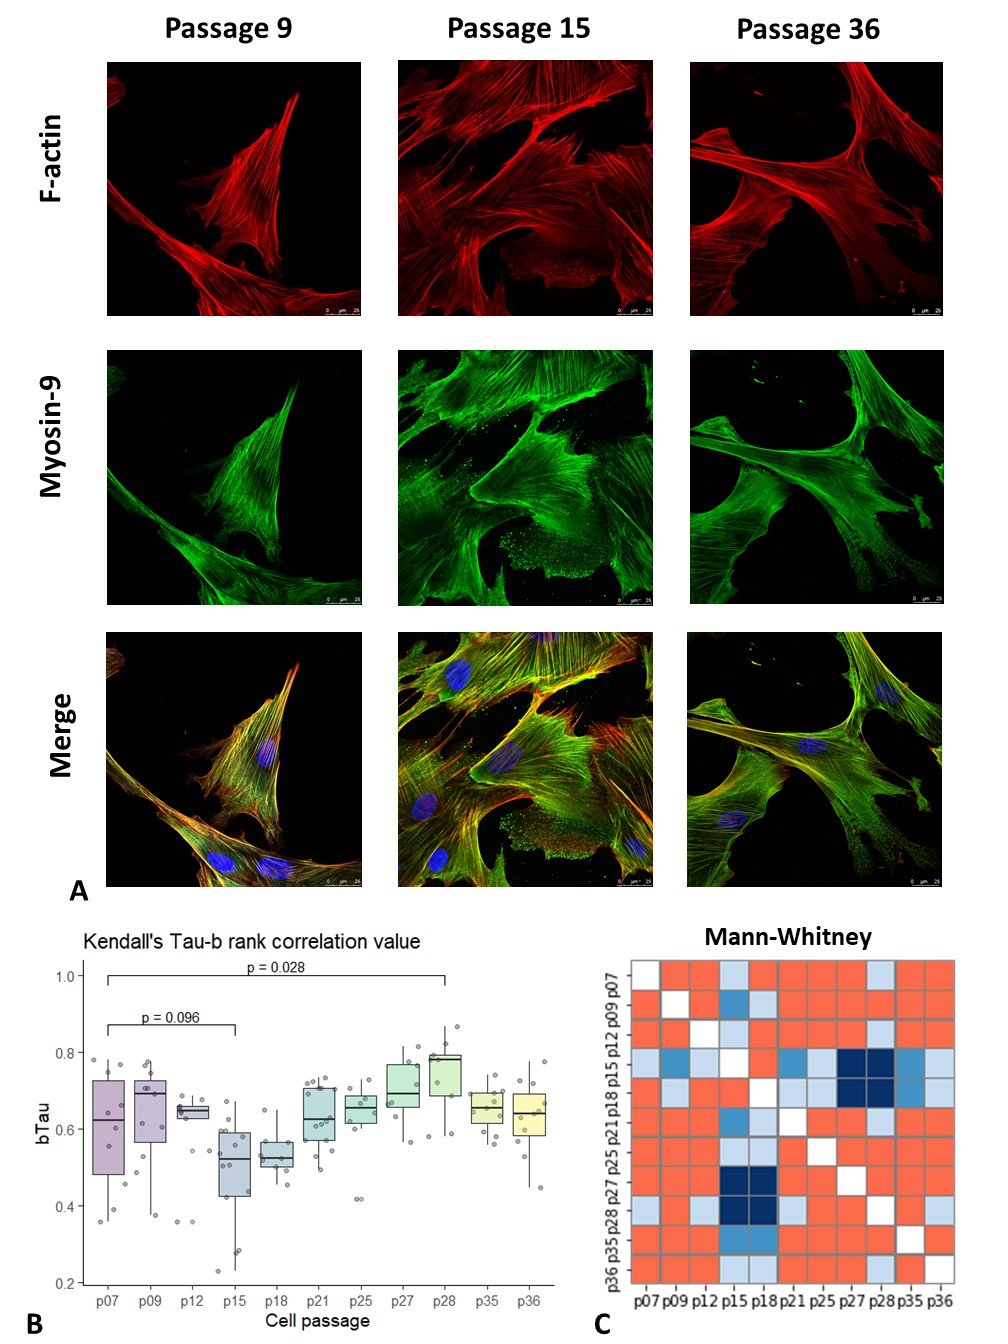
\includegraphics[width=0.9\linewidth]{myosin-9.jpg}
\caption{}
\end{figure}

\begin{figure}[hbt!]
\centering
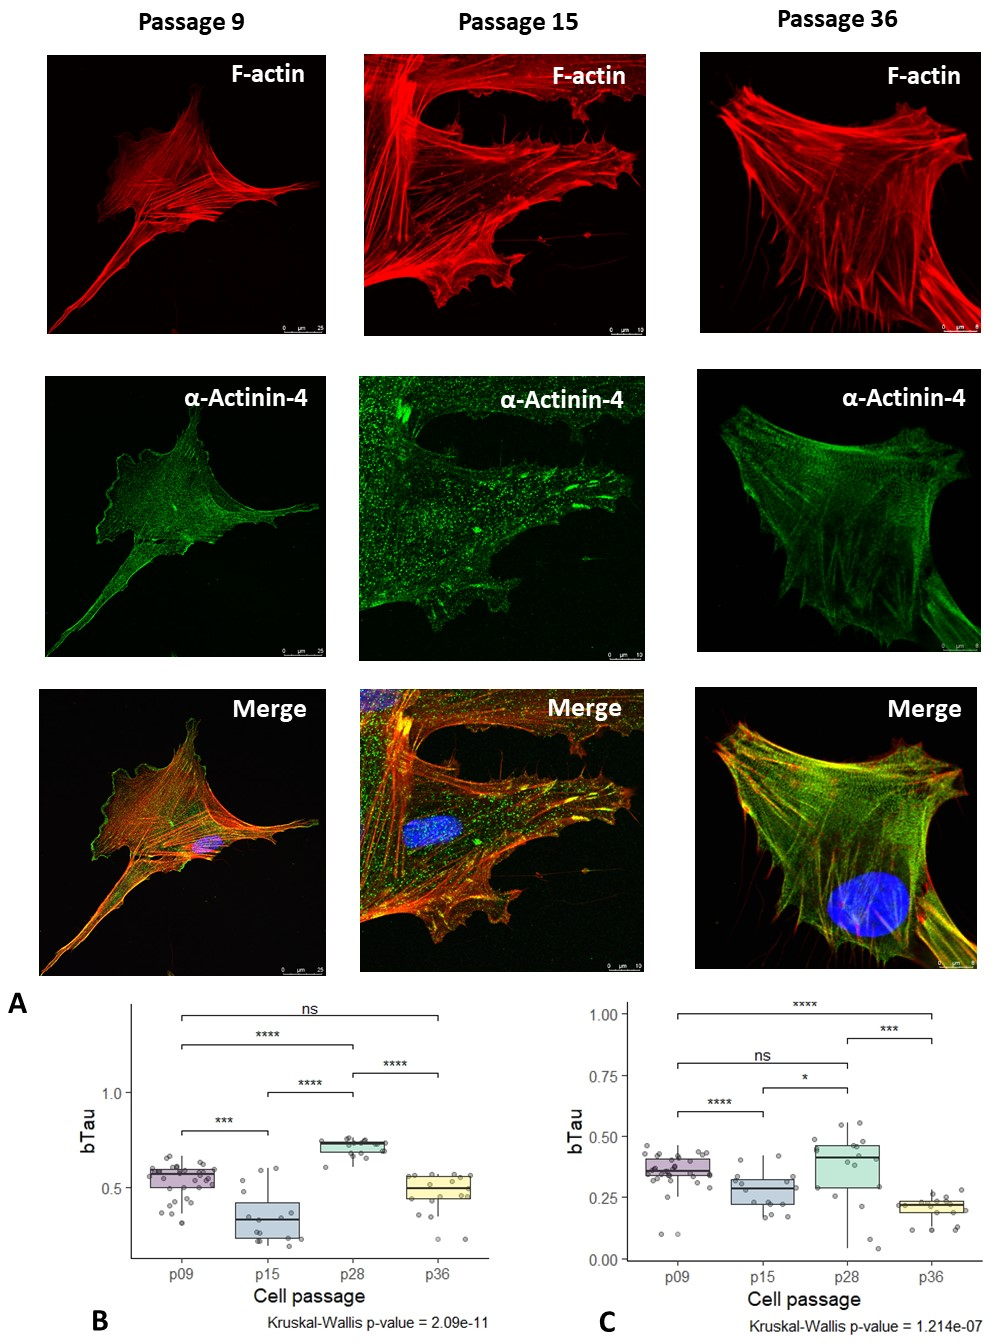
\includegraphics[width=0.9\linewidth]{alpha-actinin-4.jpg}
\caption{}
\end{figure}

\begin{figure}[hbt!]
  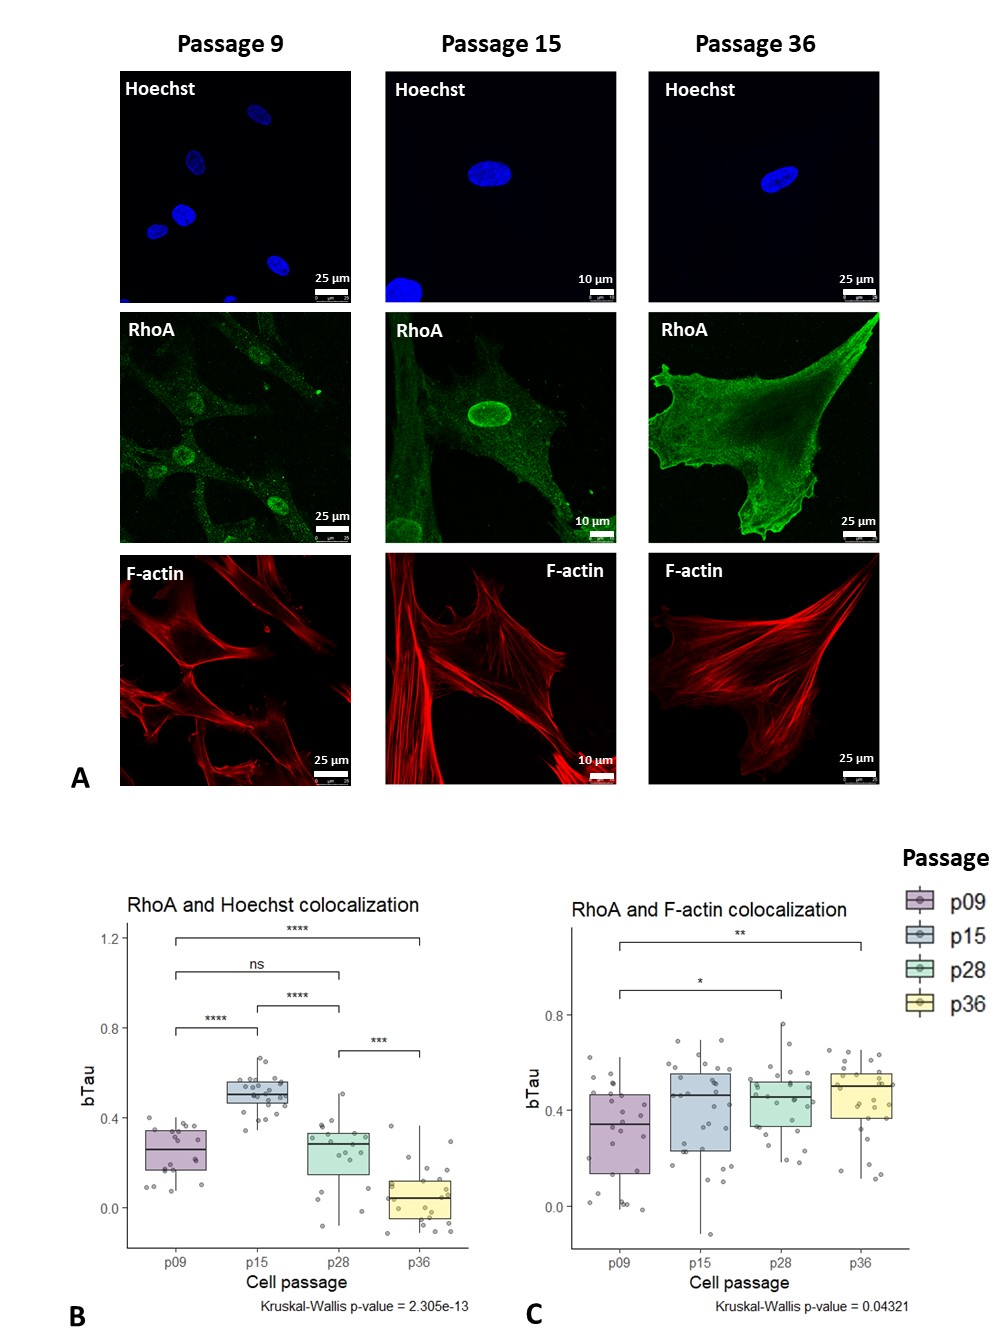
\includegraphics[width=0.9\linewidth]{rho.jpg}
  \caption{}
  \centering
\end{figure}

\begin{figure}[hbt!]
  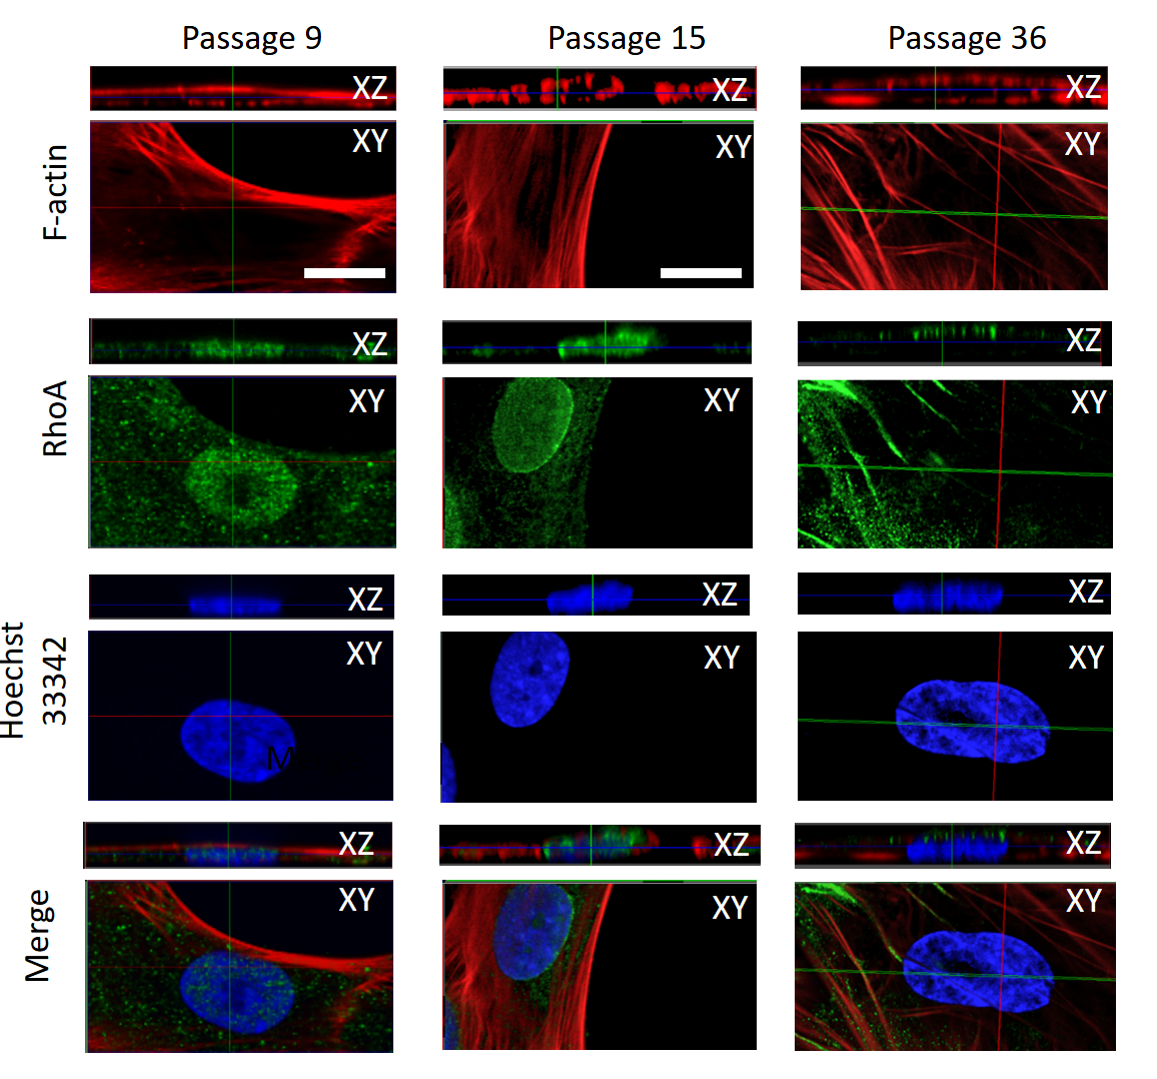
\includegraphics[width=0.9\linewidth]{rho-3d.png}
  \caption{}
  \centering
\end{figure}

\begin{figure}[hbt!]
  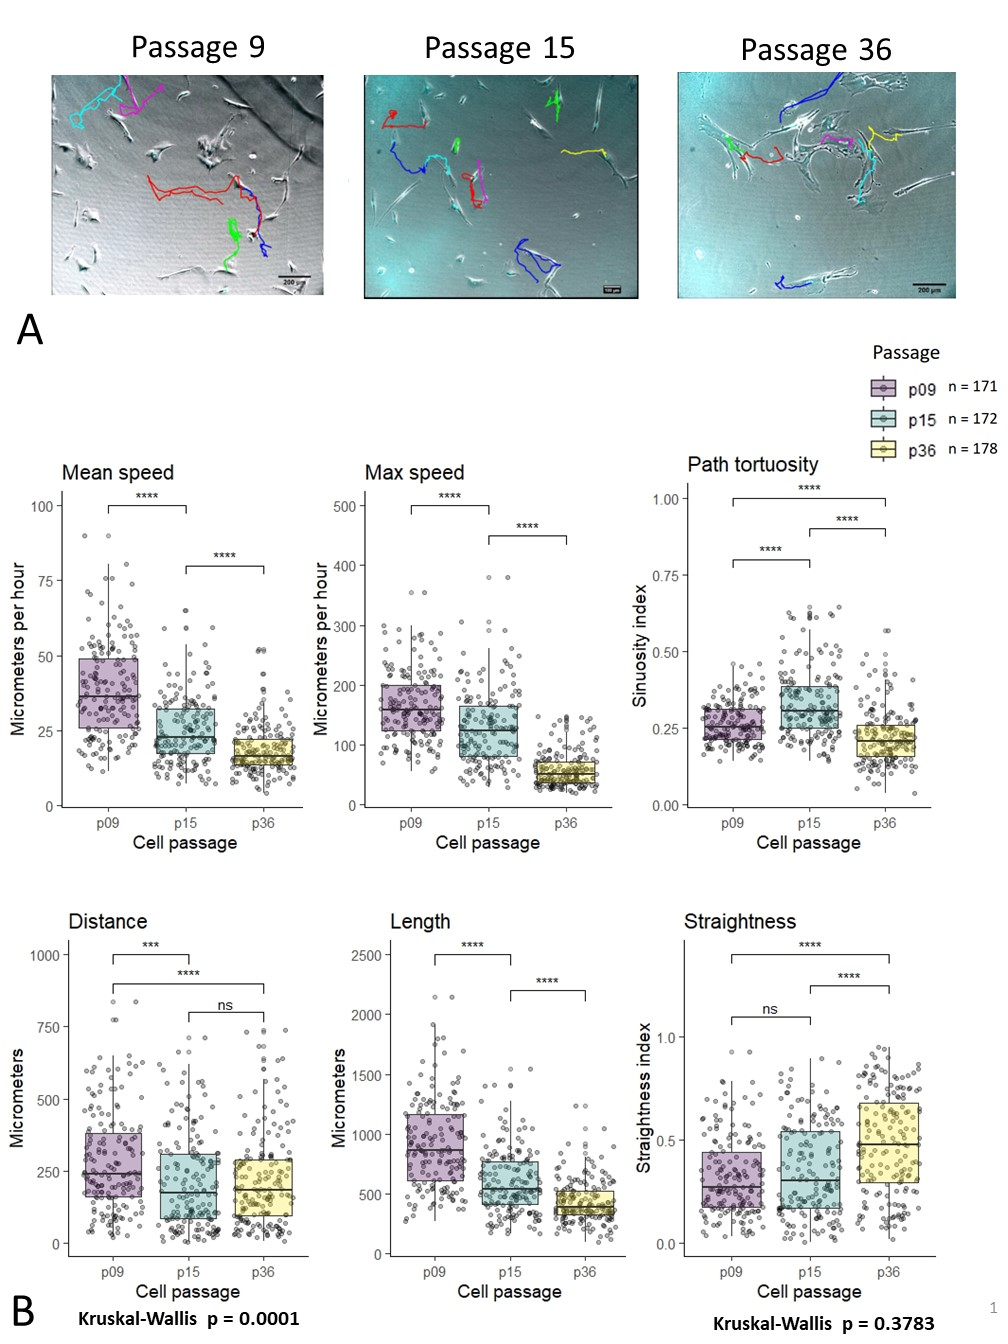
\includegraphics[width=1\linewidth]{traj.jpg}
  \caption{}
  \centering
\end{figure}

\begin{figure}[hbt!]
\centering
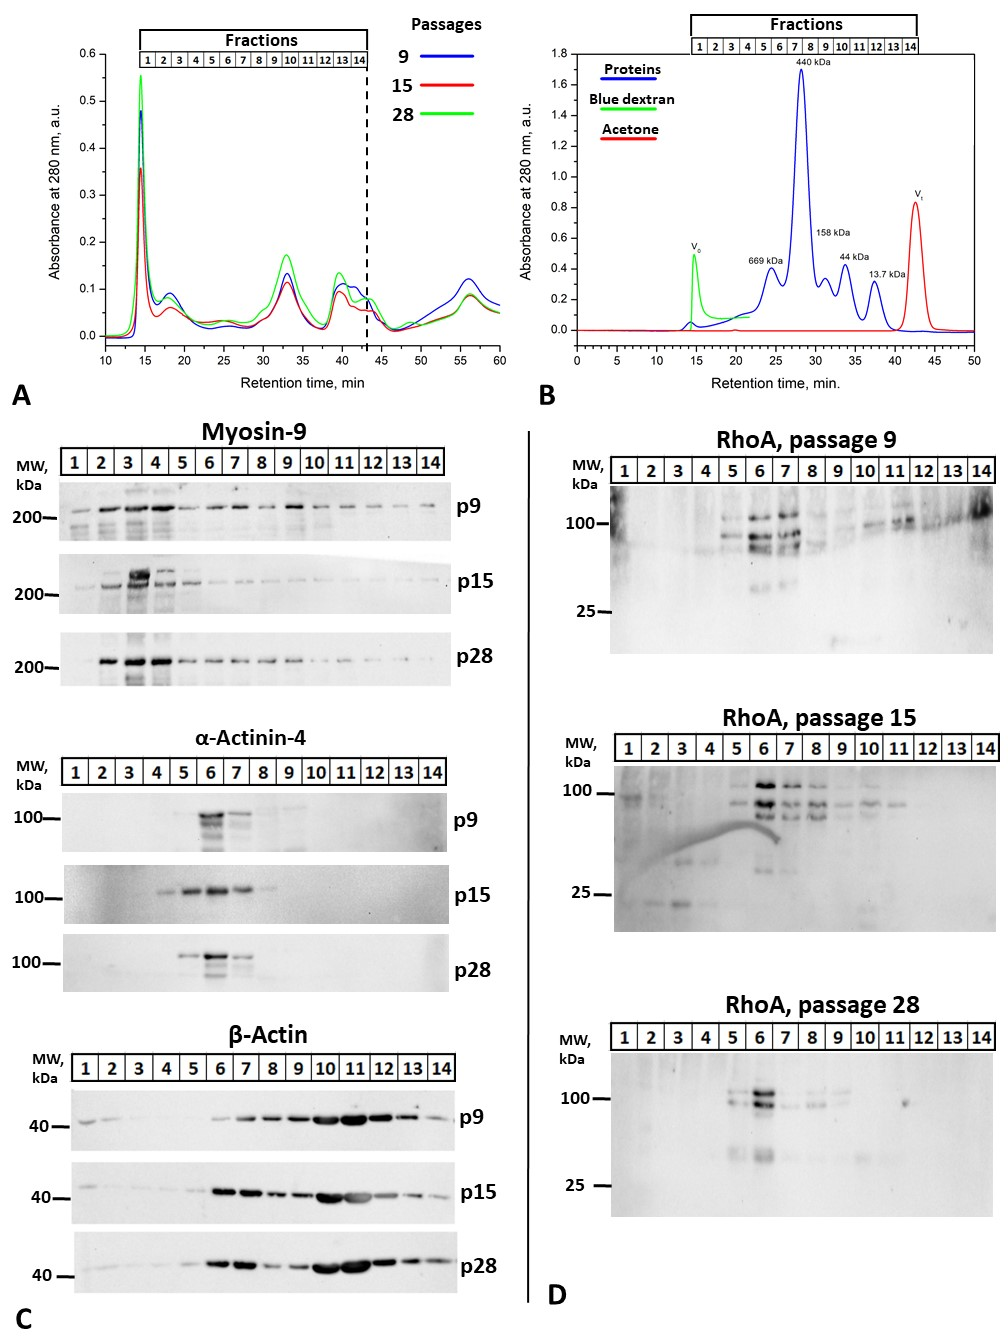
\includegraphics[width=1\linewidth]{fplc.jpg}
\caption{}
\end{figure}

%\graphicalabstract{abstract}{We provide evidence for changes in the organization of the contractile apparatus of human mesenchymal stem cells in the process of replicative senescence. The colocalization dynamics of of myosin-9 and $\alpha$-actinin-4 with F-actin, as well as RhoA with nuclei, were studied at various passages during long cultivation of mesenchymal stem cells. It was found that during replicative aging in MSCWJ-1 cells, a decline in cell speed and path tortuosity occurs.}
%\graphicalabstract{example-image-1x1}{Please check the journal's author guildines for whether a graphical abstract, key points, new findings, or other items are required for display in the Table of Contents.}Cells were fixed at passages: 7, 9, 12, 15, 18, 21, 25, 27, 28, 35, 36.

\end{document}
